\documentclass{standalone}
\usepackage{tikz}
\usetikzlibrary{shapes}
\usetikzlibrary{positioning}
\usepackage{amsmath}


\begin{document}
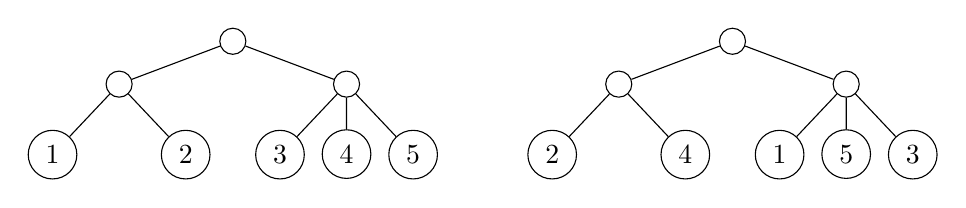
\begin{tikzpicture}[node distance=2cm]

    \node(B1)[draw, circle, minimum size=0.2cm]{};
    \node(A1)[draw, circle, minimum size=0.2cm, above right=0.3cm and 1.2cm of B1]{};
    \node(F1)[draw, circle, minimum size=0.2cm, below left=0.55cm and 0.5cm of B1]{1};
    \node(H1)[draw, circle, minimum size=0.2cm, below right=0.55cm and 0.5cm of B1]{2};

    \node(E1)[draw, circle, minimum size=0.2cm, below right=0.3cm and 1.2cm of A1]{};
    \node(I1)[draw, circle, minimum size=0.2cm, below left=0.55cm and 0.5cm of E1]{3};
    \node(G1)[draw, circle, minimum size=0.2cm, below=0.4cm of E1]{4};
    \node(K1)[draw, circle, minimum size=0.2cm, below right=0.55cm and 0.5cm of E1]{5};

    \draw (A1) -- (B1) -- (F1);
    \draw (H1) -- (B1);
    \draw (A1) -- (E1) -- (G1);
    \draw (K1) -- (E1) -- (I1);

    \node(B)[draw, circle, minimum size=0.2cm, right=6cm of B1]{};
    \node(A)[draw, circle, minimum size=0.2cm, above right=0.3cm and 1.2cm of B]{};
    \node(F)[draw, circle, minimum size=0.2cm, below left=0.55cm and 0.5cm of B]{2};
    
    \node(H)[draw, circle, minimum size=0.2cm, below right=0.55cm and 0.5cm of B]{4};

    \node(E)[draw, circle, minimum size=0.2cm, below right=0.3cm and 1.2cm of A]{};
    \node(I)[draw, circle, minimum size=0.2cm, below left=0.55cm and 0.5cm of E]{1};
    \node(G)[draw, circle, minimum size=0.2cm, below=0.4cm of E]{5};
    \node(K)[draw, circle, minimum size=0.2cm, below right=0.55cm and 0.5cm of E]{3};

    \draw (A) -- (B) -- (F);
    \draw (H) -- (B);
    \draw (A) -- (E) -- (G);
    \draw (K) -- (E) -- (I);
    



\end{tikzpicture}
\end{document}
